\documentclass[parskip,
oneside,
% 							 longdoc,
11pt,
noheadingspace,
accentcolor=tud1d,
bigchapter,
%draft,
colorback]{tudreport}


%% Spracheinstellungen
\usepackage[english]{babel}
%\usepackage[applemac]{inputenc} % Input-Encodung: applemac fuer Mac
%\IfFileExists{latin1.sty}{\usepackage{latin1}}{\usepackage{isolatin1}}
%\usepackage[latin1]{inputenc}
%\usepackage[T1]{fontenc}
\usepackage[ansinew]{inputenc}  % Input-Encodung: ansinew fuer Windows
\usepackage{microtype} % optischer Randausgleich bei pdflatex mit Zeichendehnung
\usepackage{listings}

%% Grafikeinstellungen
\usepackage{float} % u.a. genaue Plazierung von Gleitobjekten mit H
%\usepackage[latin1]{inputenc}


%% Tabelleneinstellungen
\usepackage{booktabs}
\usepackage{multirow}
\usepackage{longtable}
\usepackage{tabularx}
\usepackage{array}

%% State Chart
\usepackage{pgf}
\usepackage{tikz}
\usetikzlibrary{arrows,automata}

%% Mathematik
\usepackage{amsmath}
\usepackage{nicefrac}
\usepackage{icomma}

%% sonstige Einstellungen
\usepackage{paralist}% erweiterte Listenumgebung (z.B. compactitem)
\usepackage{textcomp} % verschiedene Symbole
\usepackage[nottoc, numbib]{tocbibind}
\usepackage{hyperref}
\renewcommand\plparsep{1ex}
\usepackage{enumerate}
\usepackage{xcolor,colortbl}
\usepackage{subfig}

\definecolor{Blue}{HTML}{9DBBE6}
\definecolor{Green}{HTML}{bfff00}

\title{\textbf{HDL Lab\\Report}}
\subtitle{Group 4\\
	Alexander Lieb - .......\\
	Blandine Riviere - 2238618}
\subsubtitle{Supervisor: Dominic Korner\hfill \\Computer Engineering Institute\hfill\textbar\hfill Integrated Electronics Systems\hfill\textbar\hfill Prof.\,Dr.-Ing.\, Klaus Hofmann}
\setinstitutionlogo{images/General/ies.pdf}

\begin{document}
	
	%% Titel %%%%%%%%%%%%%%%%%%%%%%%%%%%%%%%%%%%%%%%%%%%%%%%%%%%%%%%%%%%%%%%%%%
	\maketitle
	\cleardoublepage
	
	%% Vorgeplnkel %%%%%%%%%%%%%%%%%%%%%%%%%%%%%%%%%%%%%%%%%%%%%%%%%%%%%%%%%%%%%%
	\pagestyle{empty}
	
	%% Hauptteil %%%%%%%%%%%%%%%%%%%%%%%%%%%%%%%%%%%%%%%%%%%%%%%%%%%%%%%%%%%%%%%
	\pagestyle{headings}
	\pagenumbering{arabic}
	
	\tableofcontents
	
	\newpage
	
	\chapter*{Introduction}

% Prof. Hofmann once said, that people who are thinking that analog devices are outdated are just stupid... So I am going to change this a little bit, maybe more in his sense :)
The onset of digital age has caused a dramatic change in the conception of electronic devices. Analog and digital devices are now used to work together to fit the complex requirements of modern technology. Thus, it has become necessary to develop converters (such as Analog-Digital and Digital-Analog Converters), in order to have digital devices communicating to the outside analogic environment.\\
Concurrently, the development of digital signal processing is one of the most important fields of research, in order to meet the demand. Thus, new architectures of digital filters for subsampling, noise reduction, and so on keep emerging. One of the advantages of these filters in comparison to analog filters is the fact that they are not subject to non-linearity behavior, which considerably reduces their complexity.\\
\\
The aim of this lab was to digitally filter an analog waveform. To this end, several analog and digital components had to be implemented, such as a DAC, an ADC and a digital filter. The performance of these designs had to be evaluated with provided WAV signals. Therefore, several architectures can be compared and optimized in order to achieve better results. For this purpose, several design tools were provided, such as ModelSim for Verilog simulation, Cadence Virtuoso Analog Design Environment for mixed signals simulation and Synopsis Design Vision for Verilog module synthesis.\\
\\
This report is organized as follows. In a first part, an implementation of basic components provided as tutorial tasks is briefly described. Then, the design and performance evaluation of the developed ADC and digital filter in this lab are detailed in the second and third part respectively. Lastly, the full downsampling circuit is evaluated in the fourth part.

	
	\newpage
	
	\chapter{Basic components}

In this chapter, the first tutorial tasks, which consists in implementing an operational amplifier schematic in Cadence and a clock generator in Verilog. 

\section{Operational amplifier}

The first task is to implement an operational amplifier. The schematics of the differential stage and bias circuit of the OA are provided. The implemented amplifier is to be found in the file (\texttt{OpAmp}). The simulation results given on figure \ref{fig:opAmpSimulation} are obtained in Cadence with the following testbench (table \ref{table:opAmpTestbench}): 

\begin{table}[!h]
	\centering
	\begin{tabular}{|l|l|l|}
		\hline
		Name & Type & Value \\
		\hline
		$V_{dd}$ & constant & 1.2V \\
		$V_{ref}$, $V_{bias}$, $V_{-}$ & constant & 600mV \\
		$V_{+}$ (In) & pulse & AC=500mV, DC=0V, f=1MHz \\
		\hline
	\end{tabular}
	\label{table:opAmpTestbench}
	\caption{Operational amplifier testbench}
\end{table}

As expected, the operational amplifier is driven in a saturated operating regime and behaves as a comparator.

\begin{figure}[h]
	\centering
	\includegraphics[scale=0.65]{images/BasicComponents/Task1opAmpSimulation.png}
	\label{fig:opAmpSimulation}
	\caption{Operational amplifier simulation}
\end{figure} 

\section{Clock generator}

The second task consists in implementing a clock generator (\texttt{clkGen}) in Verilog. The Verilog code is provided. The results of the simulation in ModelSim are given on figure \ref{fig:clkGenSimulation}.

\begin{figure}[h]
	\centering
	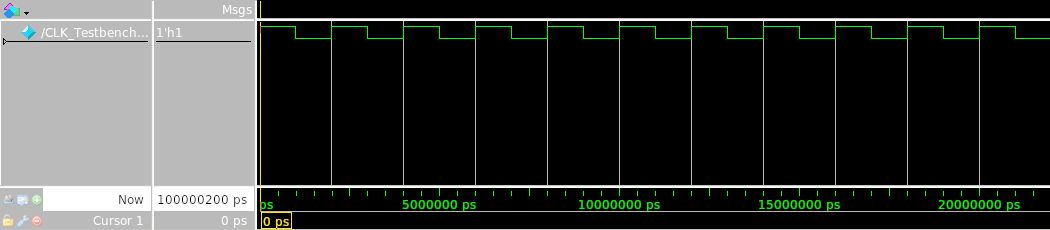
\includegraphics[scale=0.6]{images/BasicComponents/Task2ClkGenSimulation.png}
	\label{fig:clkGenSimulation}
	\caption{Clock generator simulation}
\end{figure}

For more configurability, an additional parameter \texttt{FKHZ} is introduced, which corresponds to the desired frequency in kHz.
	
	\newpage
	
	\chapter{Analog Digital Converter}

In this chapter two different versions of our ADC are getting described.

\section{Idea}

The task was to implement an 16bit ADC. We decided to implement a tracking ADC, the idea is shown in Figure ~\ref{fig:wholeADC}. This kind of ADC has different advantages, e.g. that it is choosable how good the approximation is by setting the correct frequency of the clock. Also it matches the requirements of using the DAC and the OpAmp. Our ADC is linear to the input value, which means, you can multiply the digital value with an fixed value, which depends on V\textsubscript{dd}, to get an approximation of the input value. E.g. if you are using 1.2V as V\textsubscript{dd}, you can calculate 

\[
	V_{approx} = \frac{1.2V}{2^{16} - 1} \cdot digitalValue
\]

to get the approximation of the input.

\begin{figure}[h]
	\centering
	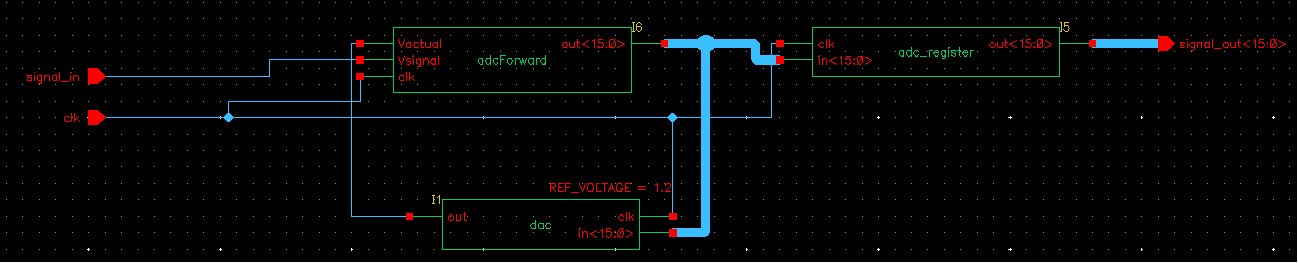
\includegraphics[scale=0.5]{images/adc/adc.png}
	\caption{the high-level view of the ADC}
	\label{fig:wholeADC}
\end{figure} 

There were several problems encountered while implementing the ADC. Besides of performance problems of Cadence, which resulted into a slow down of the development process, the comparator misses differences at its input stages, when they are to small. This results into the fact, that the ADC is not working at a stepwidth of one, but maybe at a stepwidth of 100. If the difference at the input stage of the comparator is to small, it does not return a digital value, but something in between. To face this problem, you could use several stages of comparators, but we decided to use just one stage, to show the principial, and afterwards some ideal Verilog-A modules called \texttt{simpleADC} and \texttt{simpleADCExtended}. 

\section{First Implementation}

The first implementation uses a stepwidth which has to be choosen by the user before the ADC starts to work. This has the advantage of simplifying the ADC because it does not need a stepwdith control but it is also not able to adapt to different stepwidths. This one should be used, when the analog input is nearly known and the stepwidth should be choosen carefully.

\subsection{Design}

The interesting part of the design is the part of the ADC called ADCForward. This first implementation of the forward path is shown in figure ~\ref{fig:simpleForward}. You can see that in the first step it gets decided, if the counter shall count up, down or stall. This information gets into the counter, which processes the runtime information and uses the previous configured stepwidth, to calculate the next value. As you can see in ~\ref{fig:wholeADC} this new value gets through a feedback path, containing a DAC, back to the forward path and the first part of the forward path can decide again, if the actual value is to high, so count down, to low, so count up or matching, so stop counting.

\begin{figure}[h]
	\centering
	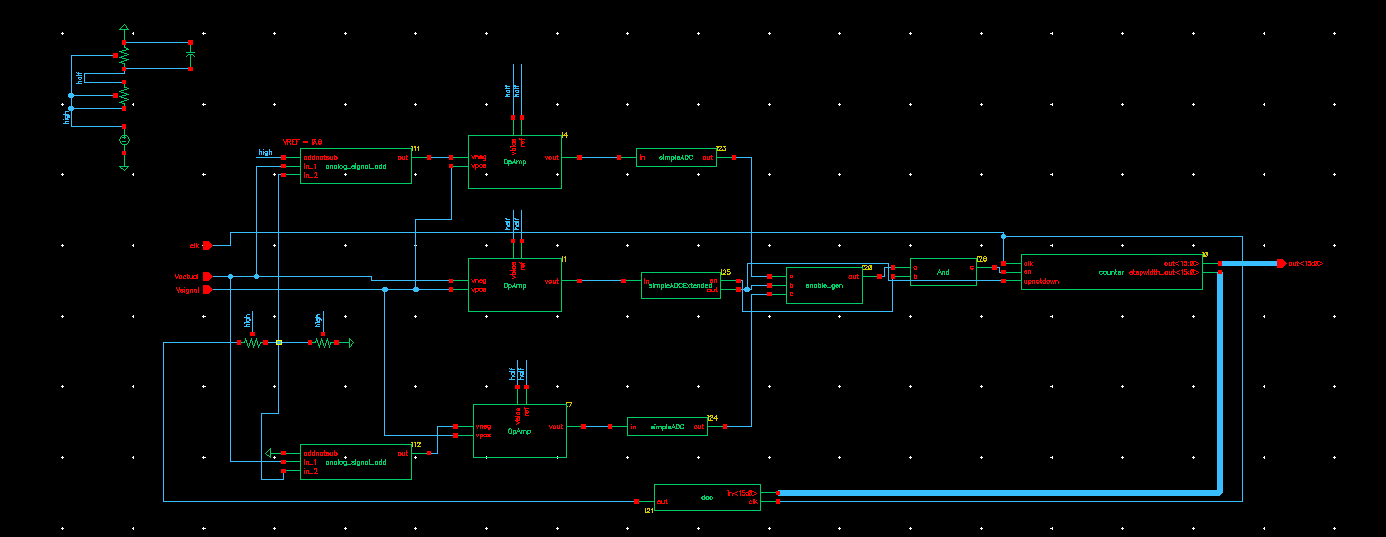
\includegraphics[scale=0.45]{images/adc/adcForward.png}
	\caption{the simple adc forward path}
	\label{fig:simpleForward}
\end{figure}

\subsection{Evaluation}

As result of the evaluation task, we got the diagram provided in figure ~\ref{fig:simpleAdcEvaluation}, using a stepwidth of 4500. The requested values can be found at table ~\ref{table:valuesSimpleADC}. Due to Cadence performance problems, the differential and integral non-linearity (DNL/INL) of the ADC could not be evaluated.

\begin{figure}[!h]
	\centering
	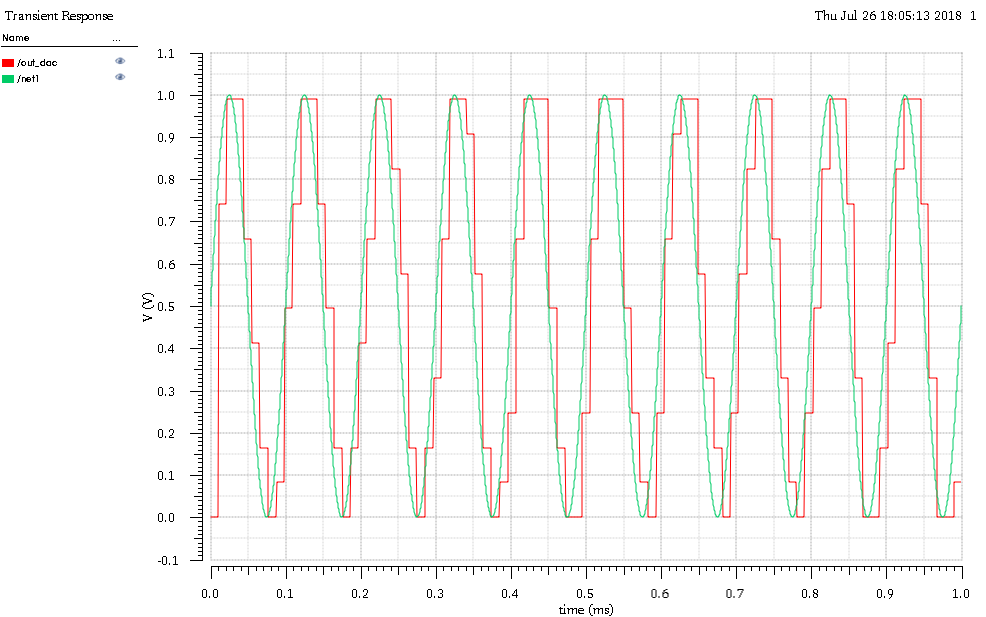
\includegraphics[scale=0.475]{images/adc/10KHzInputStepWidth4500.png}
	\caption{10kHz input and stepwidth 4500}
	\label{fig:simpleAdcEvaluation}
\end{figure}

\begin{table}[!h]
	\centering
	\begin{tabular}{|l|l|}
		\hline
		Name & Value \\
		\hline
		Maximal Sampling Frequency & 100kHz \\
		ENOB & 1.576225 bits \\
		SINAD & 11.251875 dB \\
		SNR & 11.251875 dB \\
		\hline
	\end{tabular}
	\caption{values of the simple ADC}
	\label{table:valuesSimpleADC}
\end{table}

\newpage

\section{Second Implementation}

The second implementation does not need to get a stepwidth, but calculates its own stepwidth at runtime. It is more complex, but useful, if you do not know anything about the incoming signal.

\subsection{Design}
Also here, the interesting part of the ADC is the forward path, which is called ADCForwardExtended here. This second implementation is shown in figure ~\ref{fig:extendedForward}. You can see that this forward path is divided in three steps. First, new stepwidths are getting calculated from the last choosen stepwidth. After that, the new possible values are computed and the stepwidth chooser selects the one, which is fitting best. It is also possible that the stepwdith chooser decides, that none of them are fitting good, so it keeps the last digital value and returns as used stepwidth zero.

\begin{figure}[h]
	\centering
	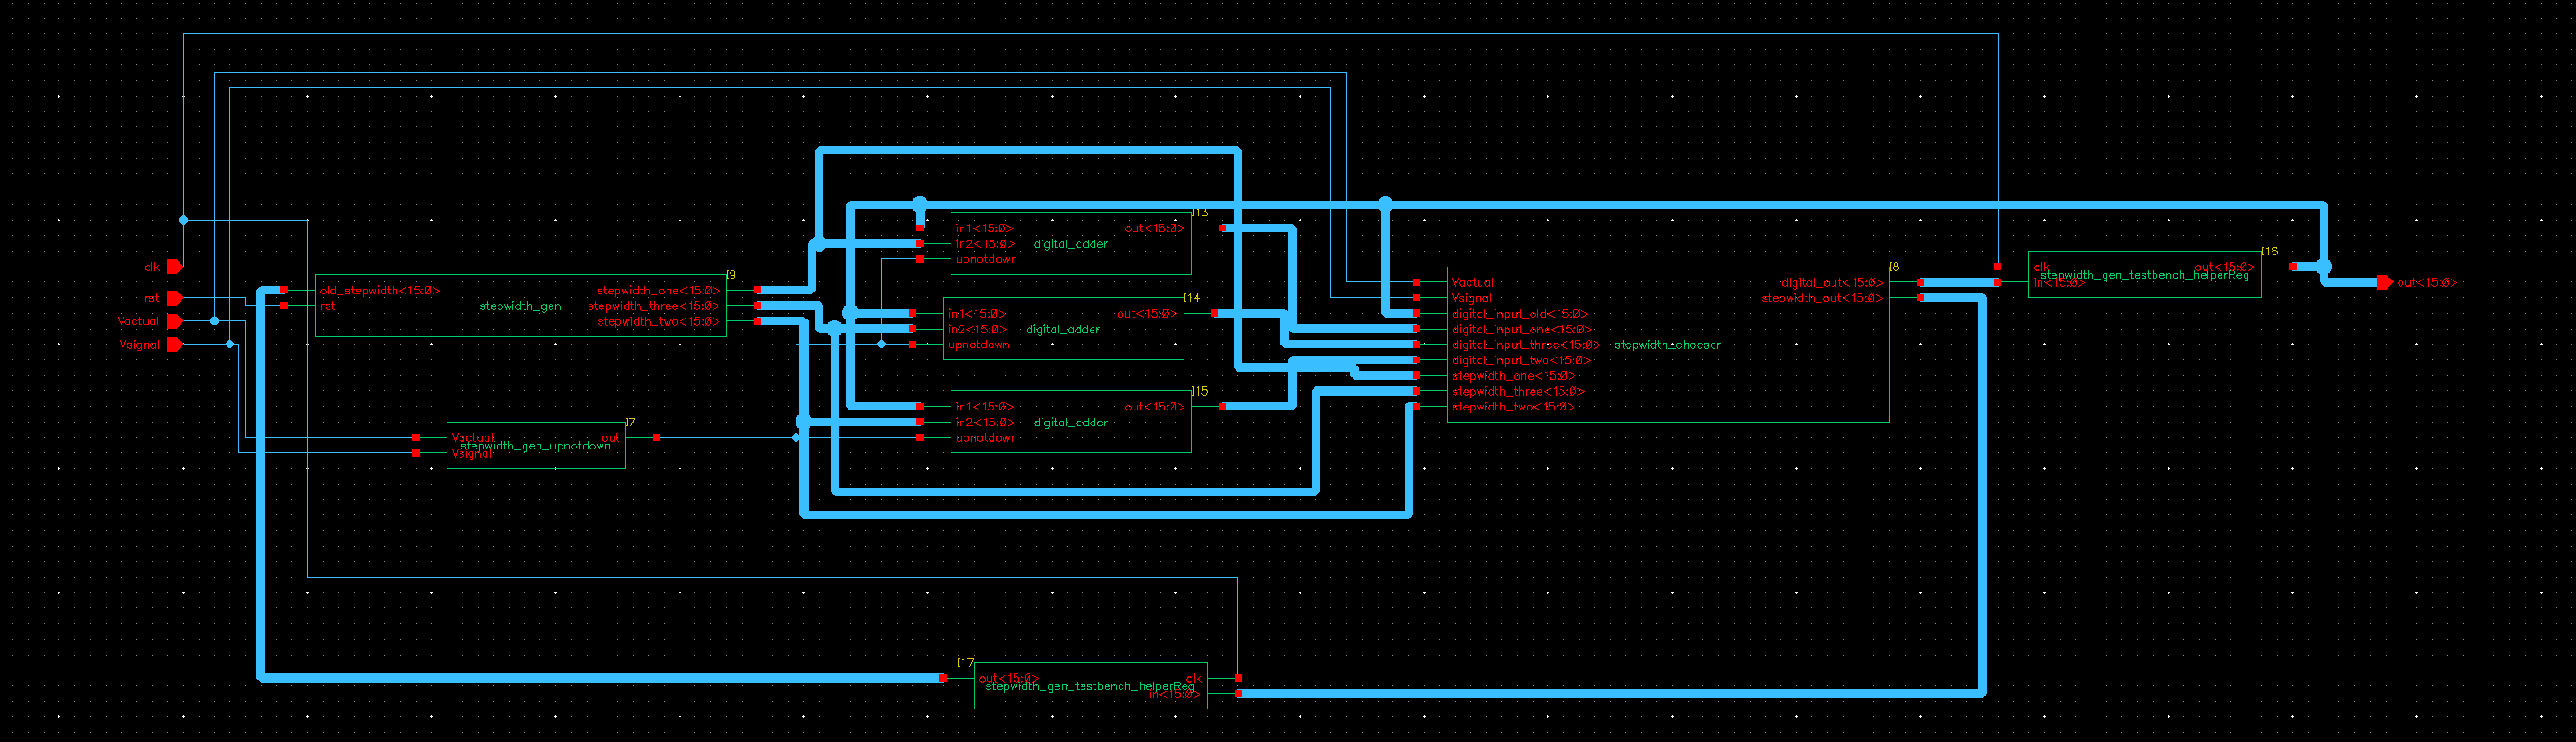
\includegraphics[scale=0.225]{images/adc/adcForwardExtended.png}
	\caption{the extended ADC forward path}
	\label{fig:extendedForward}
\end{figure}


\subsection{Evaluation}

The simulation results are shown in figure ~\ref{fig:extendedAdcEvaluation}. The requested values can be found at table ~\ref{table:valuesExtendedADC}, but here again, INL and DNL could not be computed.


\begin{figure}[h]
	\centering
	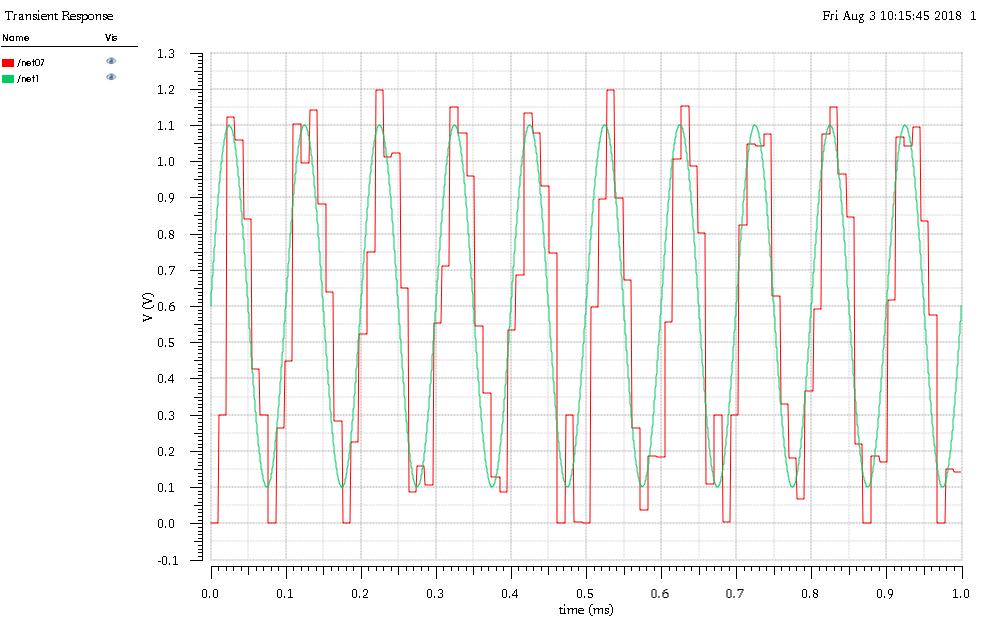
\includegraphics[scale=0.6]{images/adc/input10kHzExtended.png}
	\caption{10kHz input for the extended ADC}
	\label{fig:extendedAdcEvaluation}
\end{figure}

\begin{table}[!h]
	\centering
	\begin{tabular}{|l|l|}
		\hline
		Name & Value \\
		\hline
		Maximal Sampling Frequency & 100kHz \\
		ENOB & 1.7770844 bits \\
		SINAD & 12.461048 dB \\
		SNR & 12.461048 dB \\
		\hline
	\end{tabular}
	\caption{values of the extended adc}
	\label{table:valuesExtendedADC}
\end{table}
	
	\newpage
	
	\chapter{Digital filter}

In this chapter, the design of the implemented filter is described, as well as the simulation results.

\section{Design}

The goal of this lab is to digitally filter a waveform sampled at 44.1kHz and downsample it to a frequency of $F_{sampling}=22.05$ kHz. To perform this subsampling, it is necessary that the signal is composed of frequencies smaller than the Nyquist frequency : 
\[ F \le F_N = \frac{F_{sampling}}{2} \] 
Thus, all frequencies higher than $ F_N = 11.025$ kHz have to be filtered out by a low pass filter.\\
\\
As it is known, an ideal low pass filter is defined by its impulse response: 
\[ h(n) = B*sinc(Bn) = B * \frac{sin(\pi Bn)}{\pi Bn} \] where \[B = 2*f_{cutoff}\]
This filter is however neither causal nor finite, and therefore not feasible. To overcome this problem, it is necessary to find a window $w(n)$, such that $h(n)*w(n)$ is finite and causal. In our case, the choice is made to use the rectangle window, for reasons of simplicity : \[ w(n) = \left\{
\begin{array}{ll}
1 & \mbox{if } \vert n \vert  \le N\\
0 & \mbox{otherwise}
\end{array}
\right. \]
where $N$ is the filter order. It is noteworthy that the order $N$ must be even. A time shift has also to be added, in order to make $h(n)*w(n)$ causal. \\
The resulting impulse response in frequency domain is given by the following formula:
\[
H(\omega) = \left\{ 
	\begin{array}{ll}
	1 & \mbox{if } \vert \omega \vert \le 2 \pi f_{cutoff} = \frac{\pi}{2}\\
	0 & otherwise
	\end{array}
	\right.
\]
where the normalized cutoff frequency is \[f_{cutoff} = \frac{11025}{44100} = \frac{1}{4}\]
This allows to compute the ideal filter cofficients, which correspond to the inverse discrete Fourier transform of the impulse response:
\[
h_d^*(n) = \frac{1}{2\pi} \int H(\omega) e^{j\omega n} d\omega = \frac{1}{2\pi} \int_{-\frac{\pi}{2}}^{\frac{\pi}{2}} e^{j \omega n} d\omega = \frac{\pi}{2}  \frac{sin(\frac{\pi}{2} n)}{\frac{\pi}{2} n}
\]
Finally, the formula adopted for the implementation of the digital filter is as follows:

\[
h(n) = \sum_{k=0}^{N} h_d(k) x(n-k)
\]

where

\[
h_d(n) = h_d^*(n-N) = \frac{\pi}{2} sinc(\frac{\pi}{2} (n-N))
\]

The filter implemented in 24 bits can be found in the Verilog module \texttt{digital\_filter}. The order can be passed as parameter, so that the coefficients can be comuted accordingly. Initially, the cutoff frequency could also be set as parameter of type \texttt{real}. However, this data type is not supported by the synthesis. That is the reason why this parameter was removed and directly included in the coefficients calculation. The same goes for the coefficients which cannot be once computed and stored as \texttt{real}, and therefore need to be recomputing for each sample.

\section{Evaluation}

\subsection{Theory}

The design is first evaluated in MATLAB, to check if the chosen architecture meets the task requirements. For this evaluation, the testbench consists of a sum of identical sinus waveforms of frequencies equally distributed between 0 and 20kHz, with a step of 1kHz. The resulting spectrums are given on figure \ref{fig:filterMatlabTestbench}. For the simulation, the order of the filter is fixed to 150.

\begin{figure}[!h]%
	\centering
	\subfloat[Original signal]{{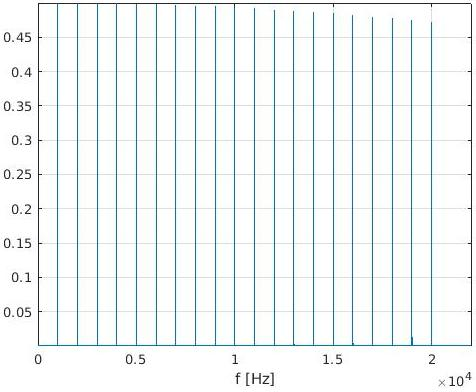
\includegraphics[scale=0.4]{images/Filter/input.jpg}}}%
	\qquad
	\subfloat[Filtered signal]{{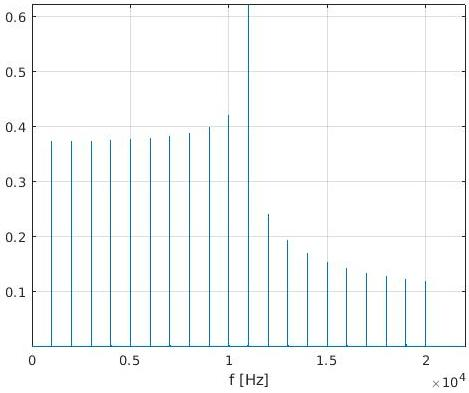
\includegraphics[scale=0.4]{images/Filter/response.jpg}}}%
	\caption{Spectrum (in magnitude) of the original and filtered signals}%
	\label{fig:filterMatlabTestbench}%
\end{figure}

As expected, the chosen filter has a low pass behavior with a cutoff frequency $F_c = 11.025 kHz$.

\subsection{Verilog implementation}

To evaluate the performance of the digital filter implemented in Verilog, a simulation is performed in Cadence. The testbench used for this purpose is to be found in \texttt{digital\_filter\_Testbench2}, and the corresponding schematic is provided in figure \ref{fig:filterTestbench}. It consists of a sum of sinus waveforms of 500Hz and 20 kHz respectively, with an offset of 2.5V, and an amplitude of 1V and 1.5V respectively. For this simulation, an ideal ADC \texttt{adc\_ideal} has been additionally implemented, to convert the analog input signal to a digital one before filtering. The values for the different parameters are given in the table \ref{table:filterTestbench}. The order of the filter is deliberately small, in order to prevent a too important delay.\\
The obtained transient waveforms and spectrums are provided respectively in figures \ref{fig:filterCadenceTestbenchTransient} and \ref{fig:filterCadenceTestbenchSpectrum}. The ENOB, SINAD and SNR values are listed in the table \ref{table:filterValues}.
 

\begin{figure}[!h]
	\centering 
	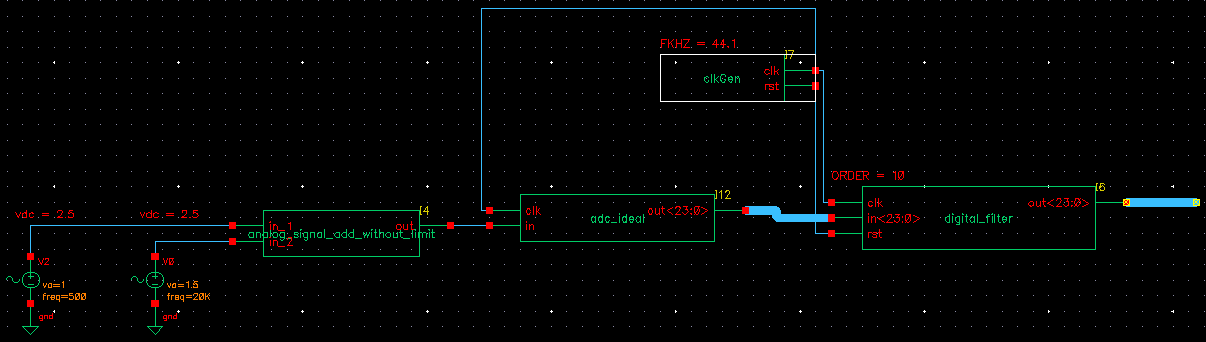
\includegraphics[scale=0.55]{images/Filter/testbench.png}
	\caption{Digital filter testbench}
	\label{fig:filterTestbench}
\end{figure} 

\begin{table}[!h]
	\centering
	\begin{tabular}{|l|r|}
		\hline
		Clock frequency (\texttt{FKHZ}) & 44.1 kHz \\
		\hline
		Filter order (\texttt{ORDER}) & 10 \\
		\hline
	\end{tabular}
	\caption{Filter testbench parameters}
	\label{table:filterTestbench}
\end{table}

\begin{figure}[!h]
	\centering 
	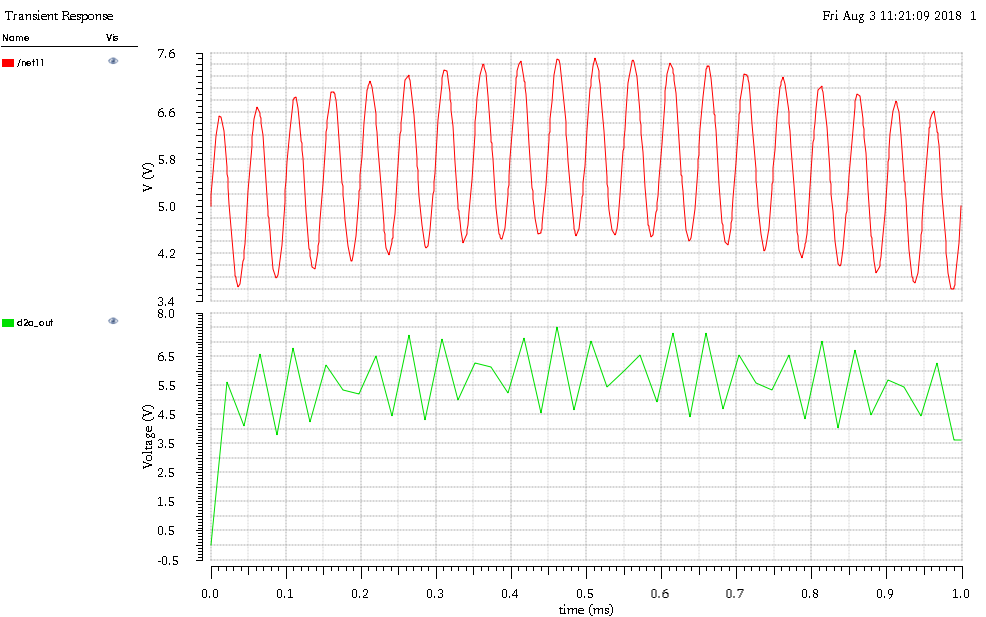
\includegraphics[scale=0.6]{images/Filter/signal.png}
	\caption{Transient simulation of the input (red) and filtered (green) signals}
	\label{fig:filterCadenceTestbenchTransient}
\end{figure} 

\begin{figure}[!h]
	\centering 
	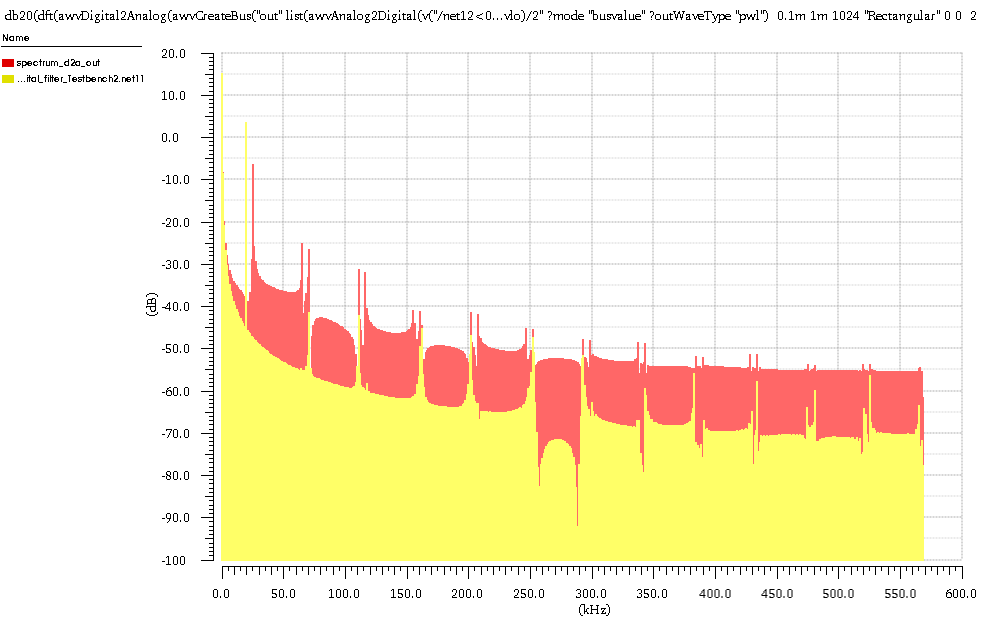
\includegraphics[scale=0.6]{images/Filter/spectrum.png}
	\caption{Spectrum of the input (yellow) and filtered (red) signals}
	\label{fig:filterCadenceTestbenchSpectrum}
\end{figure} 

\begin{table}[!h]
	\centering
	\begin{tabular}{|l|r|}
		\hline
		ENOB & -0.06092 bits \\
		\hline
		SINAD & 1.3963 dB \\
		\hline
		SNR & 1.3963 dB \\
		\hline
	\end{tabular}
	\caption{Filter statistics}
	\label{table:filterValues}
\end{table}

Surprisingly, the filtered signal contains more noise as the input signal. This may be due to the ADC which is working only at 44.1 kHz and may not capture the whole complexity of the input signal. Moreover, the relatively small order does not allow the filter to have a sharp cutoff of the higher frequencies.


\section{Synthesis}

The synthesis of the digital filter described above is performed using Synopsis Design Vision. The statistics obtained for different clock period are given in the table \ref{table:synthesisStats}.

\begin{table}[!h]
	\centering
	\begin{tabular}{|r|r|r|r|r|}
		\hline
		 \multirow{2}{*}{\textbf{Frequency}}
		 & \multirow{2}{*}{\textbf{Clock period [ns]}}
		 & \multirow{2}{*}{\textbf{Slack [ns]}} & \multicolumn{2}{c|}{\textbf{Area}} \\
		 \cline{4-5}
		 & & & \multicolumn{1}{c|}{\textbf{Cell}} & \multicolumn{1}{c|}{\textbf{Total}} \\
		\hline
		 1 GHz & 1 & - 1.78 & 31790.520257 & 54632.811374 \\
		 500 MHz & 2 & - 0.75 & 31881.240270 & 54705.954386 \\
		 \rowcolor{Blue}
		 333 MHz & 3 & 0.00 & 28362.240120 & 51198.672295 \\
		 250 MHz & 4 & 0.00 & 24488.640096 & 44641.649983 \\
		 200 MHz & 5 & 0.00 & 24275.520098 & 44453.918988 \\
		 \rowcolor{Green}
		 100 MHz & 10 & 0.00 & 23325.840074 & 41648.888715 \\
		 1 Hz & $10^{9}$ & ~$10^{9}$ & 23018.760042 & 47767.179669 \\
		\hline
	\end{tabular}
	\label{table:synthesisStats}
	\caption{Filter synthesis statistics}
\end{table} 

As shown in table \ref{table:synthesisStats}, the maximal clock frequency of the implemented filter is \textbf{333 MHz} (that is, a minimal clock period of \textbf{3 ns}). As expected, the required (cell and total) area is generally increasing with the frequency. Thus, the minimal total area is obtained for a frequency of \textbf{100 MHz}.

	
	\newpage
	
	\chapter{Downsampling circuit}

After implementing the digital filter and the Analog-Digital and Digital Analog converters, all components got integrated together in a downsampling circuit for WAV signals. The corresponding results are described in this chapter.

\section{Simple downsampling circuit}

The downsampling circuit is composed of the digital filter combined with a register, which can be found in the Verilog module \texttt{downsampling}. The task of this register is to keep only every second sample provided by the filter, in order to reduce the sampling frequency from 44.1 kHz to 22.05 kHz.\\
\\
To be able to simulate the design with WAV audio signals, additional components such as a WAV reader and a WAV writer are required. Both corresponding cell views can be found respectively in the modules \texttt{WAV\_Reader} and \texttt{WAV\_Writer}. As the read/written signals are encoded on 24 bits, as well as the filter and downsampling circuit, the connection between the 16-bit ADC and the other components is performed by a converter 24 to 16 bits (respectively 16 to 24 bits), which discards the eigth MSBs (respectively set the eight MSBs to zero). Due to the fact, that the WAV Reader and Writer only support the 16-bit WAV version, this conversion can be made without any loss of information. The corresponding modules cam be found respectively in \texttt{converterToDAC} and \texttt{converterFromADC}. 

\subsection{Simulation with sine wave signals}

For this test, the input signal is a voltage source of two added sinus waves with a DC offset of 2.5V, respective frequencies of 500 Hz and 20 kHz, and respective amplitudes of 1V and 1.5V. The corresponding schematic is provided figure \ref{fig:downsamplingSinusTestbench}. Here again, an ideal ADC is used to convert the input voltage in a digital signal. The goal of this simulation is to identify the effect of the digital filter on the input signal. Therefore, the results are stored as WAV files by means of the WAV writer, and analyzed in MATLAB. The obtained waveforms and spectrums are represented on figures \ref{fig:downsamplingSinusSignal} and \ref{fig:downsamplingSinusSpectrum}.\\
\\
\textbf{Explanation bla bla bla .... (ich mache es am Mittwoch).}


\begin{figure}[!h]
	\centering 
	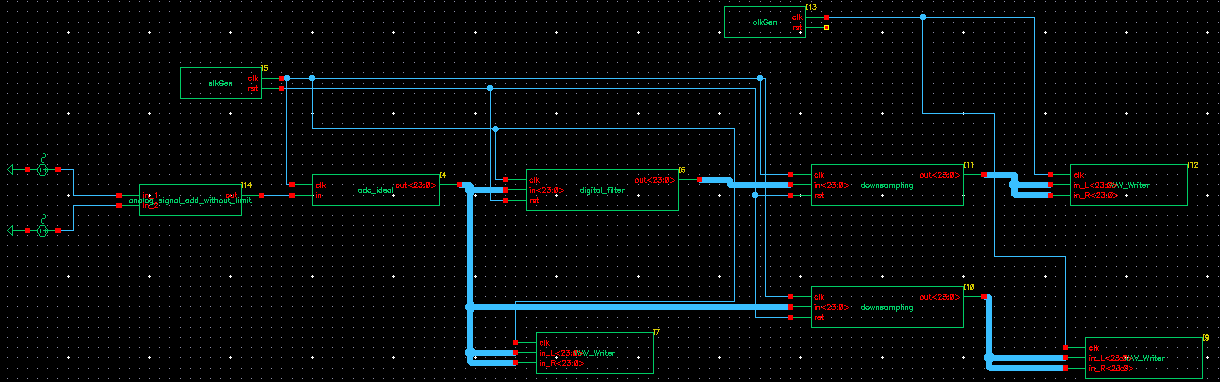
\includegraphics[scale=0.54]{images/DownsamplingCircuit/wav_downsampling_comparison.png}
	\caption{Downsampling circuit testbench (sinusoidal input voltage)}
	\label{fig:downsamplingSinusTestbench}
\end{figure} 

\begin{figure}[!h]%
	\centering
	\subfloat[Original signal]{{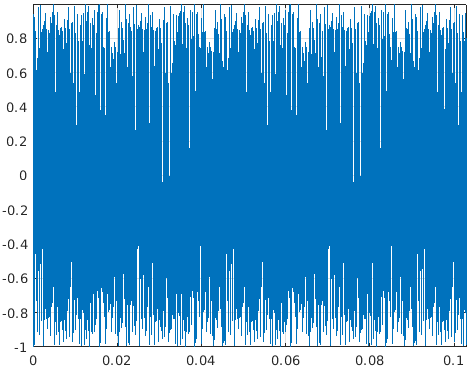
\includegraphics[scale=0.31]{images/DownsamplingCircuit/originalSignal.png}}}%
	\qquad
	\subfloat[Downsampled signal without filter]{{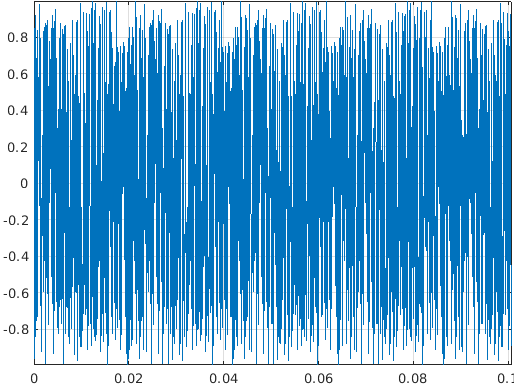
\includegraphics[scale=0.30]{images/DownsamplingCircuit/ohneFilterSignal.png}}}%
	\qquad
	\subfloat[Downsampled signal with filter]{{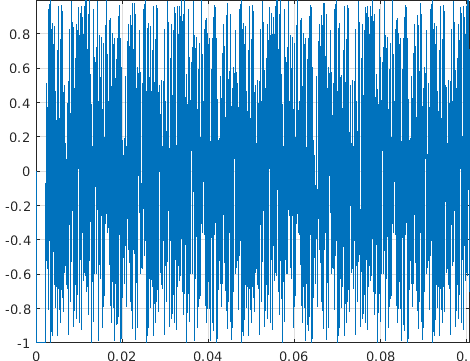
\includegraphics[scale=0.31]{images/DownsamplingCircuit/mitFilterSignal.png}}}%
	\caption{Transient simulation of the original and downsampled signals}%
	\label{fig:downsamplingSinusSignal}%
\end{figure}

\begin{figure}[!h]%
	\centering
	\subfloat[Original signal]{{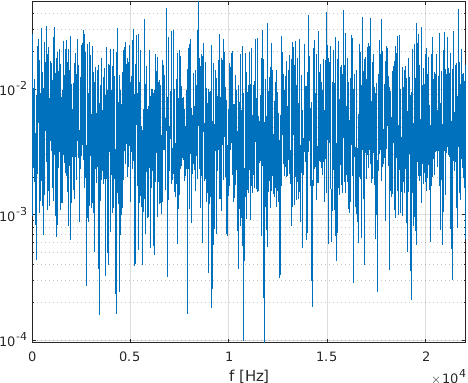
\includegraphics[scale=0.31]{images/DownsamplingCircuit/originalSpectrum.png}}}%
	\qquad
	\subfloat[Downsampled signal without filter]{{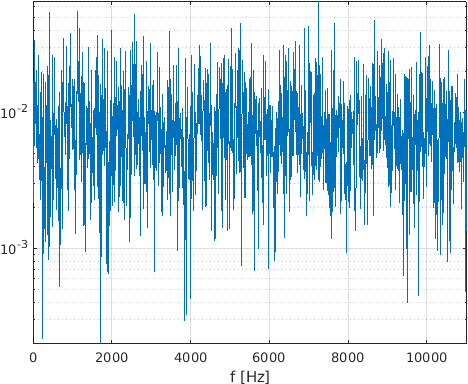
\includegraphics[scale=0.31]{images/DownsamplingCircuit/ohneFilterSpectrum.png}}}%
	\qquad
	\subfloat[Downsampled signal with filter]{{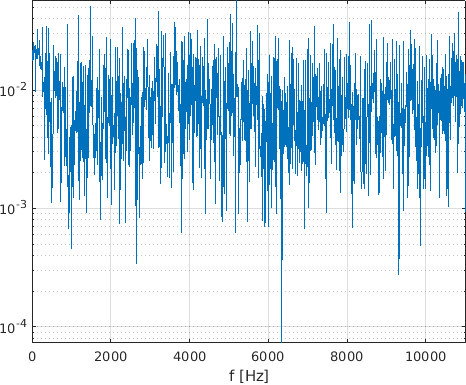
\includegraphics[scale=0.31]{images/DownsamplingCircuit/mitFilterSpectrum.png}}}%
	\caption{Spectrums (in magnitude) of the original and downsampled signals}%
	\label{fig:downsamplingSinusSpectrum}%
\end{figure}

\subsection{Simulation with audio signals}

\textbf{Text bla bla bla (ich mache es am Mittwoch).Ich habe die bilder fuer den zweiten Signal (Ex 2) rausgenommen, sonst waere es zu viele Bilder gewesen... Soll ich eher ein Channel oder doch lieber den zweiten Signal weglassen?}

\begin{figure}[!h]%
	\centering
	\subfloat[Input signal (L and R channels)]{
		\begin{minipage}{\linewidth}
			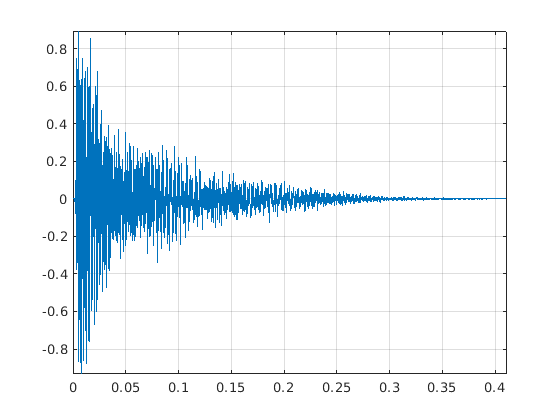
\includegraphics[scale=0.45]{images/DownsamplingCircuit/inputL.png}
			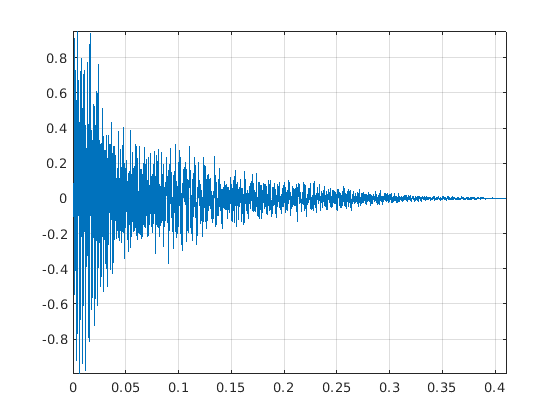
\includegraphics[scale=0.45]{images/DownsamplingCircuit/inputR.png}
		\end{minipage}
	}%
	\qquad
	\subfloat[Downsampled signal (L and R channels)]{
		\begin{minipage}{\linewidth}
			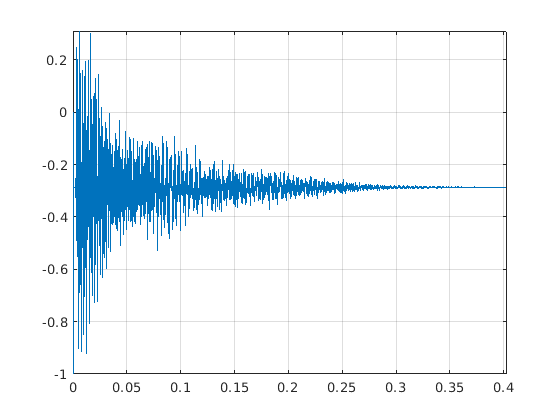
\includegraphics[scale=0.45]{images/DownsamplingCircuit/outputL.png}
			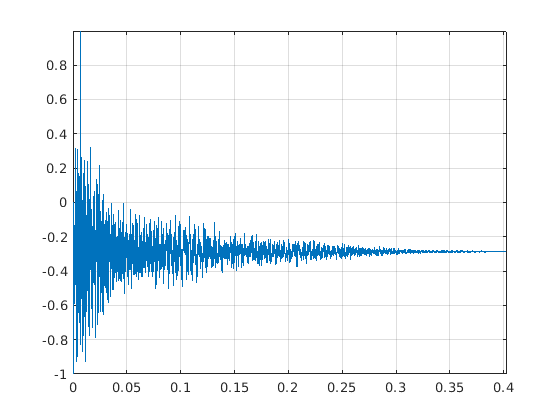
\includegraphics[scale=0.45]{images/DownsamplingCircuit/outputR.png}
		\end{minipage}
	}%
	\caption{Transient waveforms of the original and downsampled signals (Example 1)}%
	\label{fig:downsamplingWavEx1Signal}%
\end{figure}

\begin{figure}[!h]%
	\centering
	\subfloat[Input signal (L and R channels)]{
		\begin{minipage}{\linewidth}
			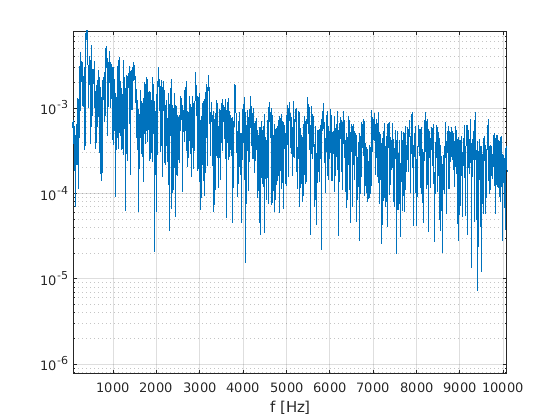
\includegraphics[scale=0.45]{images/DownsamplingCircuit/inLFFT.png}
			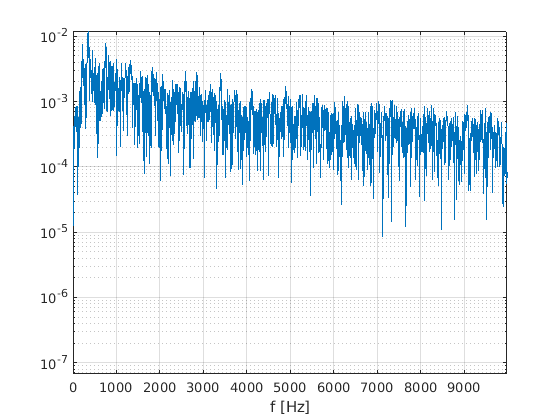
\includegraphics[scale=0.45]{images/DownsamplingCircuit/inRFFT.png}
		\end{minipage}
	}%
	\qquad
	\subfloat[Downsampled signal (L and R channels)]{
		\begin{minipage}{\linewidth}
			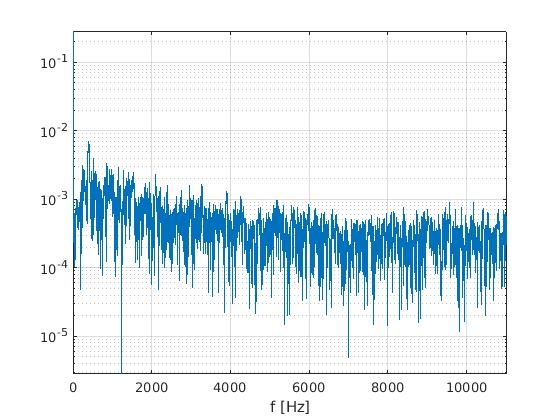
\includegraphics[scale=0.45]{images/DownsamplingCircuit/outLFFT.png}
			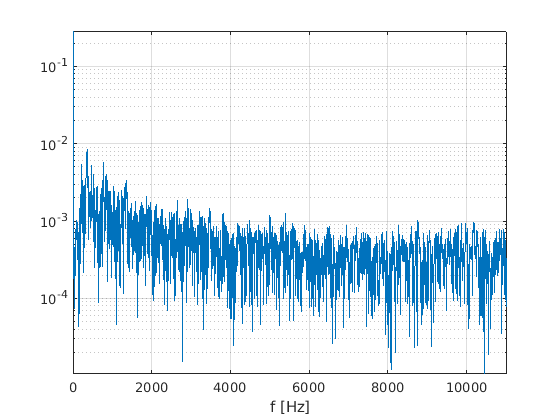
\includegraphics[scale=0.45]{images/DownsamplingCircuit/outRFFT.png}
		\end{minipage}
	}%
	\caption{Spectrum (in magnitude) of the original and downsampled signals (Example 1)}%
	\label{fig:downsamplingWavEx1Spectrum}%
\end{figure}

%\begin{figure}[!h]%
%	\centering
%	\subfloat[Input signal (L and R channels)]{
%		\begin{minipage}{\linewidth}
%			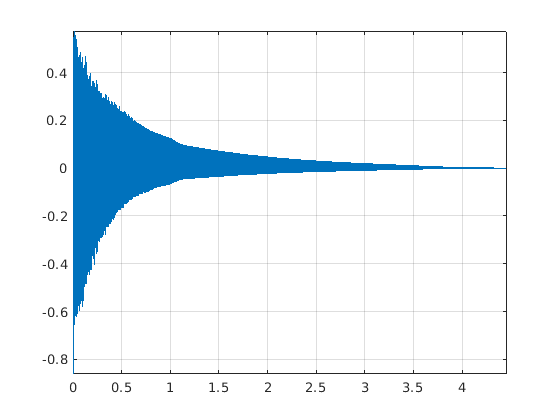
\includegraphics[scale=0.45]{images/DownsamplingCircuit/inputLEx2.png}
%			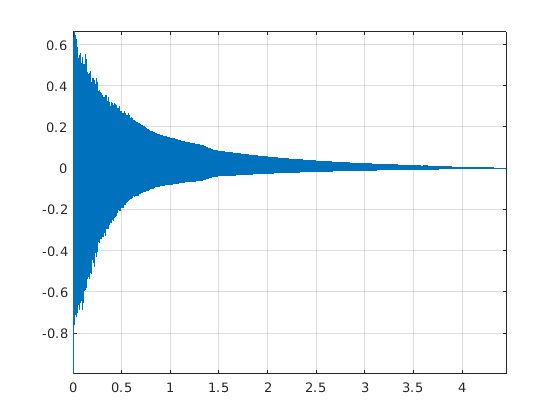
\includegraphics[scale=0.45]{images/DownsamplingCircuit/inputREx2.png}
%		\end{minipage}
%	}%
%	\qquad
%	\subfloat[Downsampled signal (L and R channels)]{
%		\begin{minipage}{\linewidth}
%			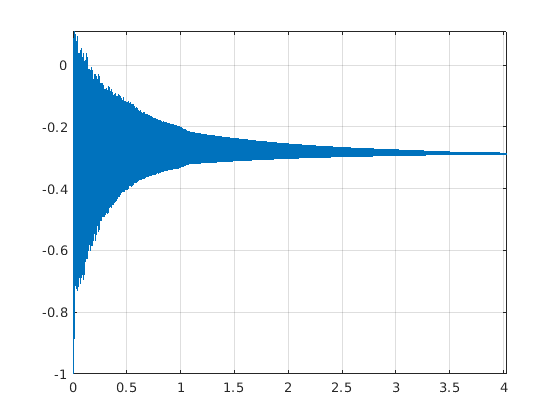
\includegraphics[scale=0.45]{images/DownsamplingCircuit/outputLEx2.png}
%			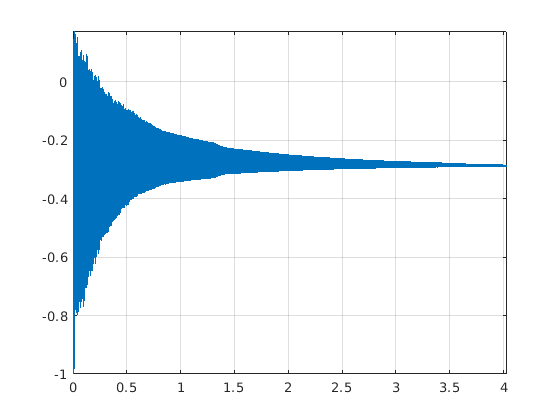
\includegraphics[scale=0.45]{images/DownsamplingCircuit/outputREx2.png}
%		\end{minipage}
%	}%
%	\caption{Transient waveforms of the original and downsampled signals}%
%	\label{fig:downsamplingWavEx2Signal}%
%\end{figure}

%\begin{figure}[!h]%
%	\centering
%	\subfloat[Input signal (L and R channels)]{
%		\begin{minipage}{\linewidth}
%			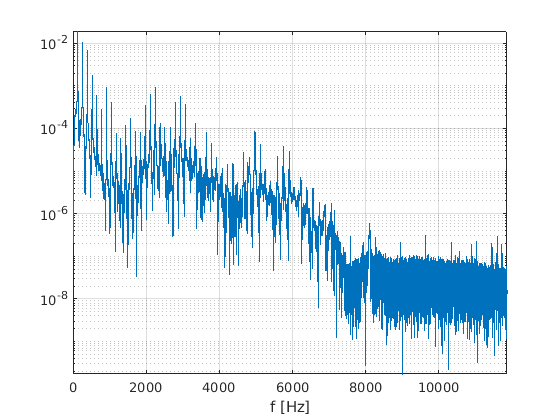
\includegraphics[scale=0.45]{images/DownsamplingCircuit/inLFFTEx2.png}
%			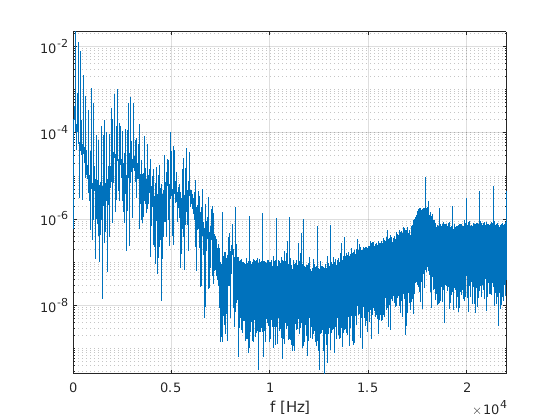
\includegraphics[scale=0.45]{images/DownsamplingCircuit/inRFFTEx2.png}
%		\end{minipage}
%	}%
%	\qquad
%	\subfloat[Downsampled signal (L and R channels)]{
%		\begin{minipage}{\linewidth}
%			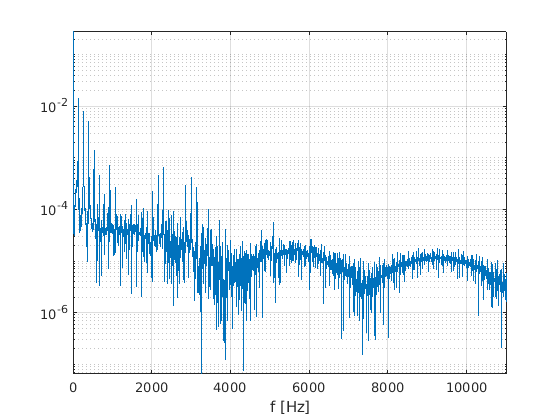
\includegraphics[scale=0.45]{images/DownsamplingCircuit/outLFFTEx2.png}
%			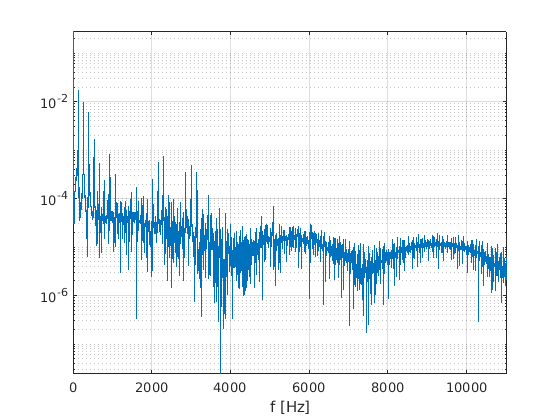
\includegraphics[scale=0.45]{images/DownsamplingCircuit/outRFFTEx2.png}
%		\end{minipage}
%	}%
%	\caption{Spectrum (in magnitude) of the original and downsampled signals (Example 2)}%
%	\label{fig:downsamplingWavEx2Spectrum}%
%\end{figure}


\section{Integration of ADC and DAC}

\textbf{Text bla bla bla (ich mache es am Mittwoch)}

\begin{figure}[!h]
	\centering 
	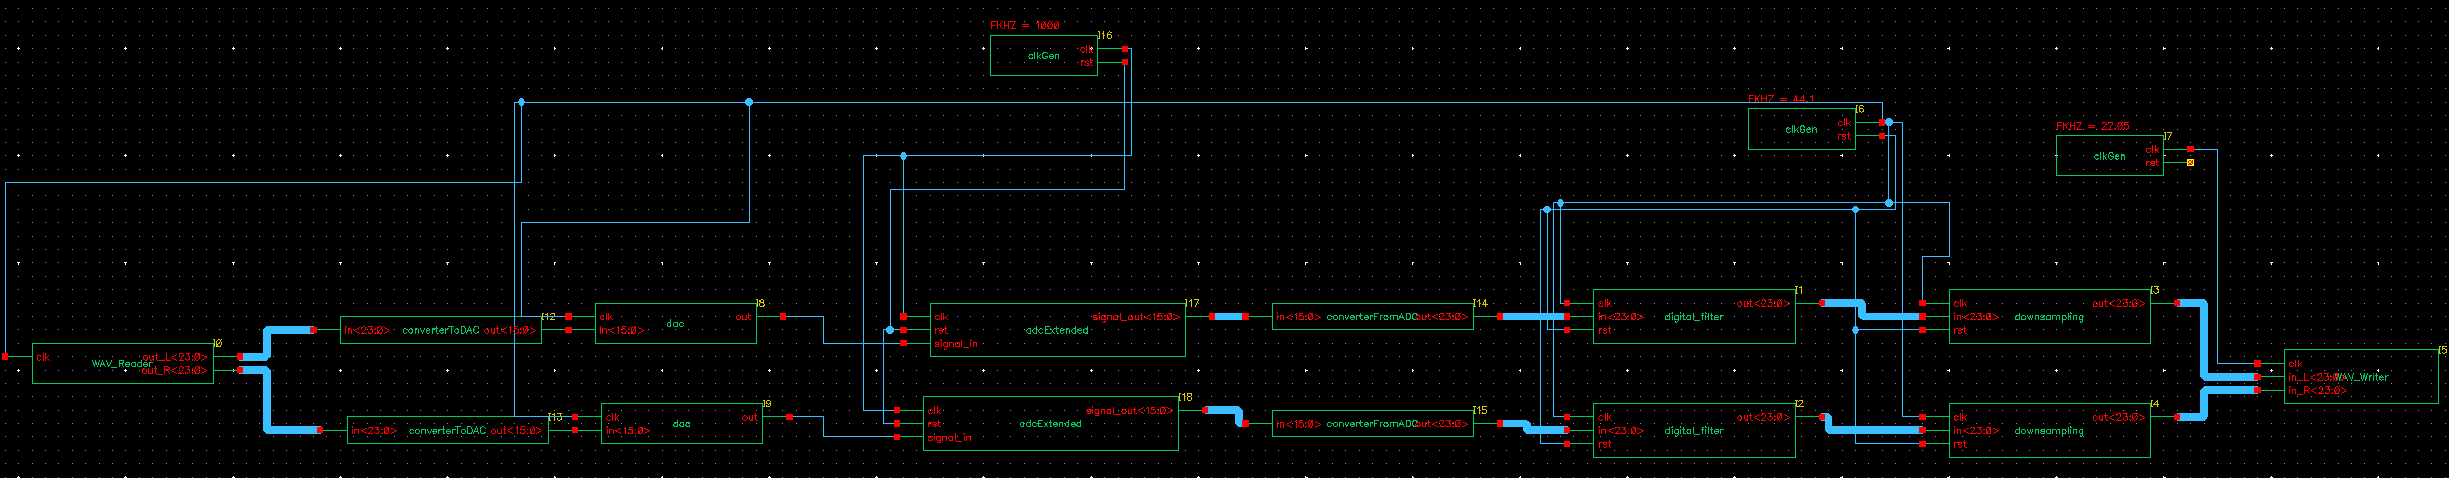
\includegraphics[scale=0.27]{images/DownsamplingCircuit/wav_downsampling.png}
	\caption{Downsampling circuit testbench (with real ADC)}
	\label{fig:downsamplingADCTestbench}
\end{figure}



	
\end{document}